I förra kapitlet togs en differentialekvation fram som beskriver vårt system som en relation mellan insignalen och utsignalen. Utifrån denna differentialekvation kan nu olika systemegenskaper tas fram som gör det möjligt att analysera systemet. Vi kommer få olika slags system med olika egensakper beroende på vilka  systemparametrar som väljs. Systemparametrarna i vårt fall är massan $m$, fjäderkonstanten $k$ och dämpningskonstanten $c$. Exempelvis kommer linan svänga olika beroende på vikten av personen på linan. 

Systemanalysen kommer titta närmare på följande funktioner: systemfunktionen, impulssvaret, stegsvaret, frekvensfunktionen samt amplitud- och faskaraktäristiken. Vissa av dessa är funktioner som existerar i tidsdomänen och andra i frekvensdomänen. Eftersom det är grundläggande att förstå hur dessa rum förhåller sig till varandra kommer detta diskuteras kort i nästa kapitel.

\newpage
\subsection{Frekvensdomänen}
Tidigare i rapporten har vi betraktat insignalen och utsignalen som funktioner av tid. Vi kommer nu även betrakta hur signalerna beter sig i frekvensdomänen där man istället kollar på vilka frekvenser en signal är uppbyggd av.

Exempelvis kan signalen $x(t)=3sin(2t) + sin(4t)$ ses som summan av två amplituder i tidsdomänen. I frekvensdomänen skulle den dock vara uppdelad i dess frekvenskomponenter, i detta fall två komponenter vid frekvenserna $2$ och $4$. Detta visas grafiskt i figuren nedan.

\begin{figure}[h] % h = here
    \centering
    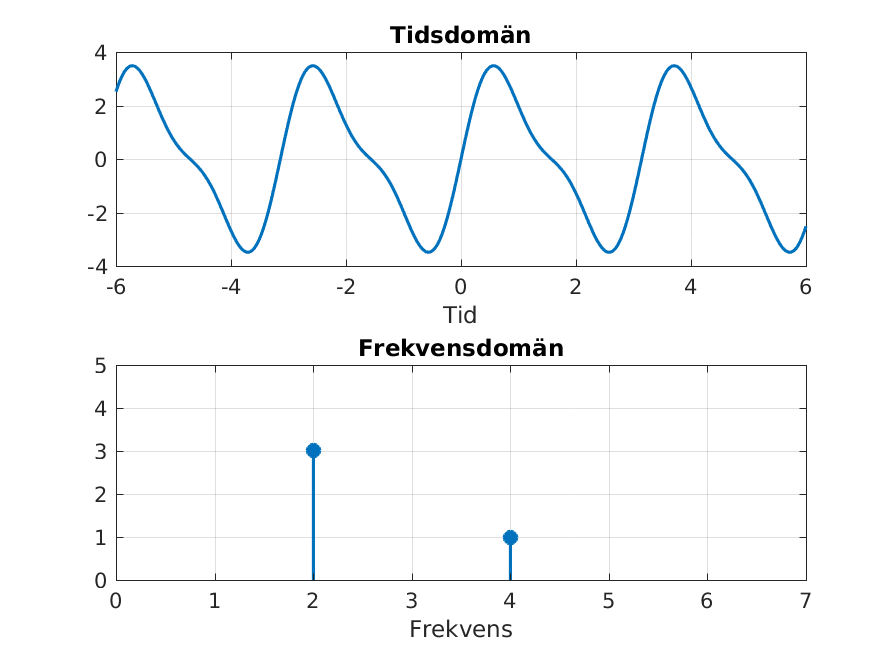
\includegraphics{bilder/tid_vs_frekvens_exempel}
    \caption{Tidsdomänen och frekvensdomänen av signalen $x(t)=3sin(2t)+sin(4t)$}
    \label{fig:tid_vs_frekvens_exempel}
\end{figure}

För systemanalysen kommer olika transformer som överför funktioner från tidsdomänen till frekvsensdomänen att användas, speciellt Laplacetransformen och Fouriertransformen.
Laplacetransformen är ett vanligt verktyg för att lösa differentialekvationer. För att ta sig tillbaka till tidsdomänen från frekvensdomänen kan inverstransformer appliceras.

\subsection{Systemfunktion}
Systemfunktionen $H(s)$ beskriver förhållandet mellan utsignalen och insignalen i frekvensdomänen. Detta betyder att man kan räkna ut en utsignal om man vet insignalen i frekvensdomänen och systemfunktionen. 
Detta går också att göra i tidsdomänen med faltning men det är oftast enklare att utföra beräkningen i frekvensdomänen.

För att beräkna systemfunktionen kommer hela differentialekvationen för systemet att Laplacetransformeras till frekvensdomänen. Det finns då två versioner av Laplacetransformen som kan användas: den enkelsidiga och den dubbelsidiga.
Eftersom vårt system är kausalt, alltså att utsignalen inte beror på på framtida insignaler så kommer den enkelsidigia transformen att användas.
Den enkelsidiga Laplacetransformen för en funktion $x(t)$ definieras som:
$$X(s) = \mathcal{L}\big\{x(t)\big\} = \int\limits_{0-}^{\infty} x(t)e^{-st}\,dt$$
där s är en komplexvärd frekvens vanligtvis betecknad $s=\sigma+j\omega$.
Här används versaler för att beteckna funktioner i frekvensdomänen.
Denna transform behöver inte vara definierad för alla $s$ utan kan divergera i vissa fall. Därför är det viktigt att säga var den transformerade funktionen är definierad. 

Eftersom dessa integralberäkningar kan bli både långa och krångliga kommer vi i denna rapport använda tabellerna i häftet \textit{Formler \& Tabeller}\footnote{Sune Söderkvist, \textit{Formler \& Tabeller}, 4:e upplagan (2007)} för att beräkna Laplacetransformerna.
För att transformera differentialekvationen kommer följande samband för derivering i tidsdomänen att användas enligt tabell 18.7:
$$\mathcal{L}\bigg\{\frac{dy(t)}{dt}\bigg\} = sY(s)-y(0-)$$
Då vårt system är energifritt är alla $y(0-)$-termer lika med noll. Vår differentialekvation kan alltså Laplacetransformeras enligt:
$$ \mathcal{L}\bigg\{m\displaystyle\frac{d^2y(t)}{dt^2} + c\displaystyle\frac{dy(t)}{dt} + ky(t)\bigg\}= \mathcal{L}\bigg\{x(t)\bigg\} $$
\begin{center}$ \Longleftrightarrow \bigg/$ Tabell $18.7$, $18.8\,\bigg/$ \end{center}
$$ \Longleftrightarrow\, ms^2Y(s)+csY(s)+kY(s)=X(s)$$

Från ekvationen ovan kan nu systemfunktionen $H(s)$ bestämmas då den definieras som kvoten mellan utsignalen och insignalen i frekvensdomänen. Genom att bryta ut termen $Y(s)$ i vänsterledet och sedan dela med $X(s)$ och $s$-polynomet i båda led ges följande: 
$$H(s)=\frac{Y(s)}{X(s)}=\frac{1}{ms^2+cs+k}$$
\newline

\subsubsection{Pol-nollställediagram}
Utifrån systemfunktionen kan nu flera egenskaper om systemet tas fram. Oftast är det intressant att studera nollställena för polynomen i systemfunktionen. Täljarpolynomets rötter kallas systemfunktionens nollställen medan nämnarpolynomets rötter kallas systemfunktionens poler. Man kan direkt se att systemfunktionen inte har några nollställen då täljarpolynomet inte har några rötter. För att hitta polerna måste rötterna till nämnarpolynomet hittas, detta kan till exempel göras med pq-formeln:
$$ms^2+cs+k=0$$
$$\Longleftrightarrow s=-\frac{c}{2m}\pm \sqrt{\bigg(\frac{c}{2m}\bigg)^2-\frac{k}{m}}$$

Här uppstår 3 potentiella fall för poler beroende på uttrycket i kvadratroten, den så kallade diskriminanten.

\begin{itemize}
    \item Om diskriminanten är positiv bildas två skilda reella poler. Kravet är då: 
    $$ \bigg(\frac{c}{2m}\bigg)^2-\frac{k}{m} > 0 \,\,\, \Longleftrightarrow\,\,\, \frac{c^2}{4m} > k $$   
    \item Om diskriminanten är noll bildas en reell dubbelpol. Kravet för dubbelpolen är: 
    $$ \bigg(\frac{c}{2m}\bigg)^2-\frac{k}{m} = 0 \,\,\, \Longleftrightarrow\,\,\, \frac{c^2}{4m} = k $$
    \item Om diskriminanten är negativ bildas två komplexkonjugerade poler. Kravet för komplexa poler är: 
    $$ \bigg(\frac{c}{2m}\bigg)^2-\frac{k}{m} < 0 \,\,\, \Longleftrightarrow\,\,\, \frac{c^2}{4m} < k $$
\end{itemize}

Som nämnts innan behöver inte Laplacetransformen vara definierad för alla $s$. Var transformen konvergerar i det komplexa planet bestäms av den reella delen av $s$ och kallas konvergensområdet. För kausala system får man högersidiga konvergensområden i det komplexa planet. Då bestäms konvergensområdets vänstra gräns av den pol som är längst till höger. För vårt system får vi två fall för detta beroende på var polerna är placerade.
\begin{itemize}
    \item Om vi har en reell dubbelpol eller komplexkonjugerade poler så är konvergensområdet:
    $$ Re\{s\} > -\frac{c}{2m} $$
    \item Om vi har två skilda reella poler så blir konvergensområdet:
    $$ Re\{s\} > -\frac{c}{2m}+\sqrt{\bigg(\frac{c}{2m}\bigg)^2-\frac{k}{m}} $$
\end{itemize}

För att få en bättre förståelse av systemfunktionen kommer poler, nollställen och konvergensområdet visas grafiskt i ett pol-nollställediagram. För detta behöver även nivånkonstanten $K$ bestämmas. Denna fås genom att bryta ut koefficienterna för den högsta graden av $s$ i täljar- och nämnarpolynomet. I vårt fall är denna alltid:
$$K=\frac{1}{m}$$
Nedan visas pol-nollställediagramen för de 3 olika fallen för polerna. Enligt standardnotation representerar kryssen poler och cirklar nollställen, dock uppstod inga nollställen. De rödsträckade området är konvergensområdet.

\begin{figure}[H] 
    \centering
    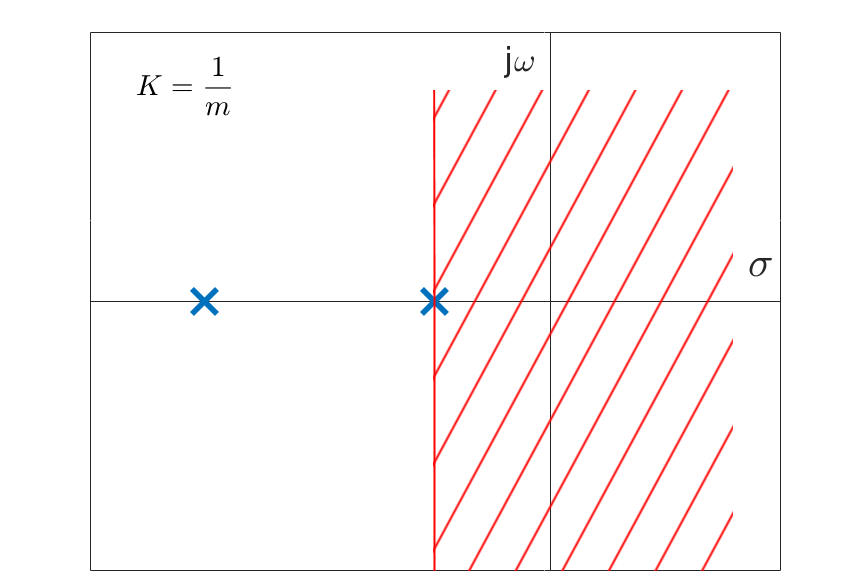
\includegraphics[scale=0.33]{bilder/pol_nollstallediagram_2_poler}
    \caption{Pol-nollställediagram för 2 skilda reella poler}
    \label{fig:pol_nollstallediagram_2_poler}
\end{figure}
\begin{figure}[H] 
    \centering
    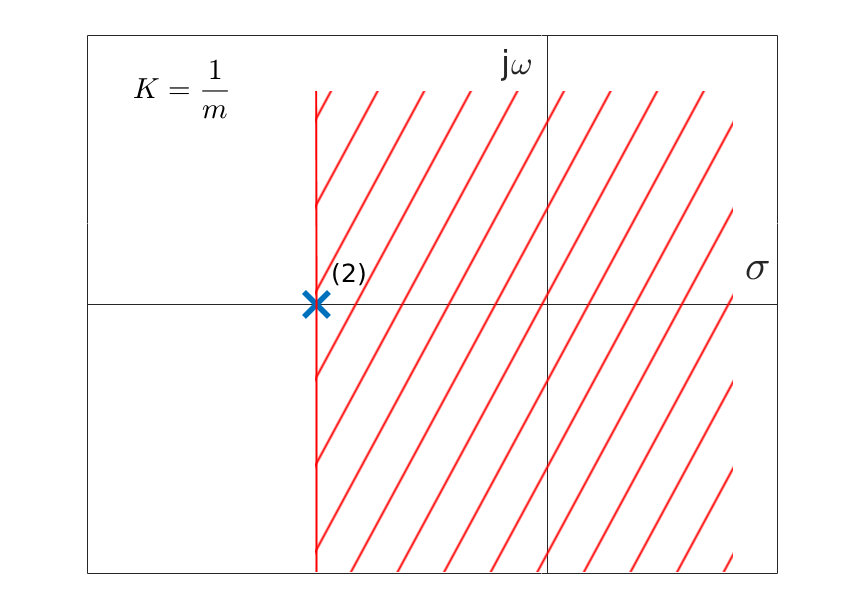
\includegraphics[scale=0.33]{bilder/pol_nollstallediagram_dubbelpol}
    \caption{Pol-nollställediagram för en reell dubbelpol}
    \label{fig:pol_nollstallediagram_dubbelpol}
\end{figure}
\begin{figure}[H] 
    \centering
    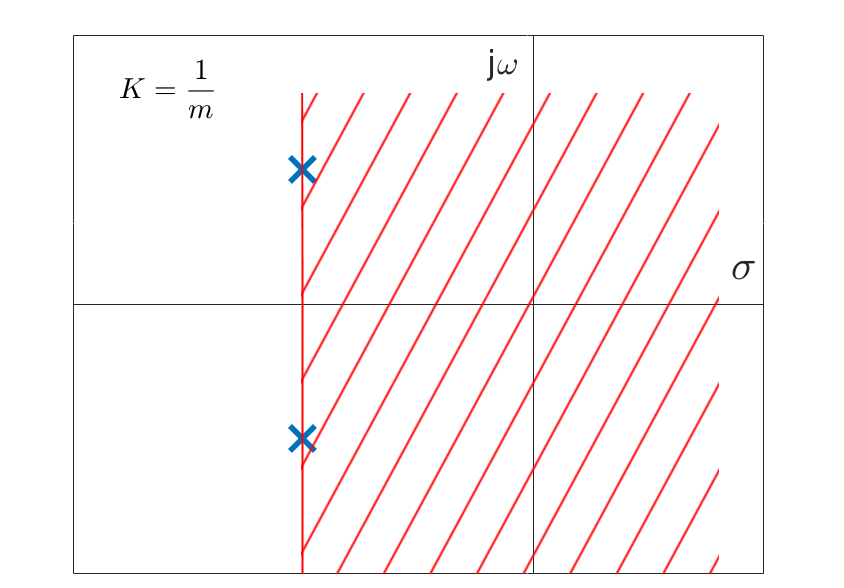
\includegraphics[scale=0.33]{bilder/pol_nollstallediagram_komplexa_poler}
    \caption{Pol-nollställediagram för två komplexkonjugerade poler}
    \label{fig:pol_nollstallediagram_komplexa_poler}
\end{figure}
 
\newpage
\subsection{Impulssvar}
Vi ska nu se hur vårt system reagerar olika på typer en insignaler. En vanligt signal som studeras är enhetsimpulsen också kallad Dirac-pulsen, $\delta(t)$. 
Enhetsimpulsen är noll för alla värden $t\ne 0$. Vid $t = 0$ är den oändligt stor så att dess area är lika med $1$. Det är svårt att föreställa hur detta skulle representera sig fysikalisk i vår modell. Ett ungefärligt exempel skulle vara då man släpper en tennisboll från en hög höjd som träffar personen på huvudet och studsar bort. 

Impulssvaret $h(t)$ är utsignalen då ett system tar emot en enhetsimpuls som insignal. Denna kan räknas ut genom att inverstransformera systemfunktionen $H(s)$. Vi kommer återigen att använda tabeller för dessa beräkningar då integralerna är jobbiga att räkna ut. Man får istället problemet att skriva om uttrycken så att de matchar något i tabellen. Då det finns tre uppsättningar av poler kommer implussvaret för dessa räknas ut separat.

\begin{itemize}
    \item Vid 2 skilda reella poler kan vi faktorisera rötterna i nämnarpolynomet och partialbråksuppdela för att hitta en lämplig inverstransform.
    
    $$H(s)=\frac{1}{m} \cdot \frac{1}{s^2+\frac{cs}{m}+\frac{k}{m}}=\Bigg/ \,\alpha=\frac{c}{2m}\,\,,\,\,\, \omega_0=\sqrt{\bigg(\frac{c}{2m}\bigg)^2-\frac{k}{m}} \,\,\Bigg/$$
    $$=\frac{1}{m} \cdot \frac{1}{\big(s+\alpha-\omega_0\big)\big(s+\alpha+\omega_0\big)}  = \, \frac{1}{2m\omega_0} \Bigg(\frac{1}{s+\alpha-\omega_0}-\frac{1}{s+\alpha+\omega_0}\Bigg)$$
    \begin{center}$ \Longleftrightarrow \bigg/$ Tabell $19.12\,\bigg/$ 
    $\Longleftrightarrow h(t)=\dfrac{1}{2m\omega_0}\bigg(e^{-(\alpha-\omega_0)t}-e^{-(\alpha+\omega_0)t}\bigg)u(t)$ \end{center}
    
    \item Vid reell dubbelpol kvadratkompletteras nämnarpolynomet och utnyttjas att
    $\dfrac{k}{m}-\dfrac{c^2}{4m^2}=0$.
    $$ H(s)= \frac{1}{m} \cdot\frac{1}{\big(s+\frac{c}{2m}\big)^2+\big(\frac{k}{m}-\frac{c^2}{4m^2}\big)} = \frac{1}{m} \cdot \frac{1}{\big(s+\frac{c}{2m}\big)^2}$$
    \begin{center}
    $ \Longleftrightarrow \bigg/ \alpha=\dfrac{c}{2m}\,,\,$ Tabell $19.15\,\bigg/ \Longleftrightarrow h(t)=\dfrac{1}{m} \cdot te^{-\alpha t}\,u(t)$
    \end{center}
    
    \item För komplexkonjugerade poler kvadratkompletteras nämnarpolynomet precis som innan. Sedan anpassas uttrycket med hjälp av förlängning för att överrensstämma med tabellen.
    $$H(s)=\frac{1}{m} \cdot \frac{1}{\big(s+\frac{c}{2m}\big)^2+\big(\frac{k}{m}-\frac{c^2}{4m^2}\big)} = \Bigg/\, \,\alpha=\frac{c}{2m}\,\,,\,\,\,\omega_0=\sqrt{\frac{k}{m}-\frac{c^2}{4m^2}} \,\,\,\Bigg/ $$
    \begin{center}
    $=\dfrac{1}{m\omega_0} \cdot \dfrac{\omega_0}{(s+\alpha)^2+\omega_0^2} \,\,\Longleftrightarrow \bigg/$ Tabell $19.23\,\bigg/\Longleftrightarrow\,\, h(t)=\dfrac{1}{m\omega_0} \cdot e^{-\alpha t} \sin(\omega_0 t)u(t)$
    \end{center}
\end{itemize}

\subsubsection{Val av systemparametrar}
För att kunna visualisera och analysera impulssvaren måste först systemparametrarna bestämmas. Dessa bestämmer hur systemen beter sig och är i vårt fall de tre hittills obestämda konstanterna massan  $m$, fjäderkonstanten $k$ och dämpningskonstanten $c$. Vi bestämmer en standarduppsättnnig för systemparametrarna. För att se hur system med olika parameteruppsättningar skiljer sig åt kommer en parameter i taget varieras medan de andra två hålls konstanta.

Valet av systemparametrar baseras på scenariot som beskrivs i inledningen. Den första parametern som kommer bestämmas är massan. Denna bestäms vara $75$ kg,  vilket är den ungefärliga medelvikten hos svenska män och kvinnor enligt Statistiska centralbyrån.
Nästa parameter är dämpningskonstanten vilket härleds från differentialekvationen i viloläget, där konstanten $k$ kan skrivas som:
\newline$$k=\frac{mg}{y_0}$$\newline
Vi måsta därför bestämma en rimlig utdragning av linan i viloläget för att sedan räkna ut $k$. Vi anser att en rimligt utdragning av linan är $0.5$ m efter att studerat bilder och filmklipp av riktiga lindansare. Vi antar att jordens tyngdacceleration $g$ kan approximeras till $9.82$. Då beräknas fjäderkonstanten till:
\newline$$k=\frac{75 \cdot 9.82}{0.5}=1473 \text{ N/m}$$

Sist har vi dämpningskonstanten $c$ som är svår att bestämma. Denna kan bestämmas till exempel experimentellt genom att mäta hur mycket systemet dämpar en insignal. Detta är inte möjligt i vårt fall och vi behöver därför resonera oss fram till ett rimligt värde. Dämpningskonstanten kommer bestämma typen av system alltså vilken typ av poler som bildas. Vi vill att systemet dämpar insingaler så lindansaren har lättare att balansera sig på linan. Man vill fortfrande ha lite gung i linan men den ska vara väldigt begränsad. Vi får denna effekt då vi har två skilda reella poler och kravet för det var:
$$\frac{c^2}{4m} > k $$
Löser vi ut $c$ och stoppar in värdena från innan får vi:
$$c>\sqrt{4km}=\sqrt{4\cdot 1473\cdot 75} \approx 665$$
Vi väljer att $c=700$ kg/s för att skapa trevliga värden när vi utför beräkningar på systemet. 

Standardparameteruppsättningen sammanställs då som:

$\begin{cases}
\begin{aligned}
m&=75 \text{ kg} \\
k&=1473 \text{ N/m} \\
c&=700 \text{ kg/s}
\end{aligned}
\end{cases}$

\newpage
\subsubsection{Variation av impulssvaret}
Vi ska nu undersöka impulssvaret grafiskt för de parametrar vi har valt och vad som händer om dessa ändras. Först är vi intresserad av hur impulssvaret beter sig med våra standardparameteruppsättning alltså att $m = 75$ kg, $k=1473$ N/m och $c=700$ kg/s. Detta visas i figuren nedan.

\begin{figure}[H]
    \centering
    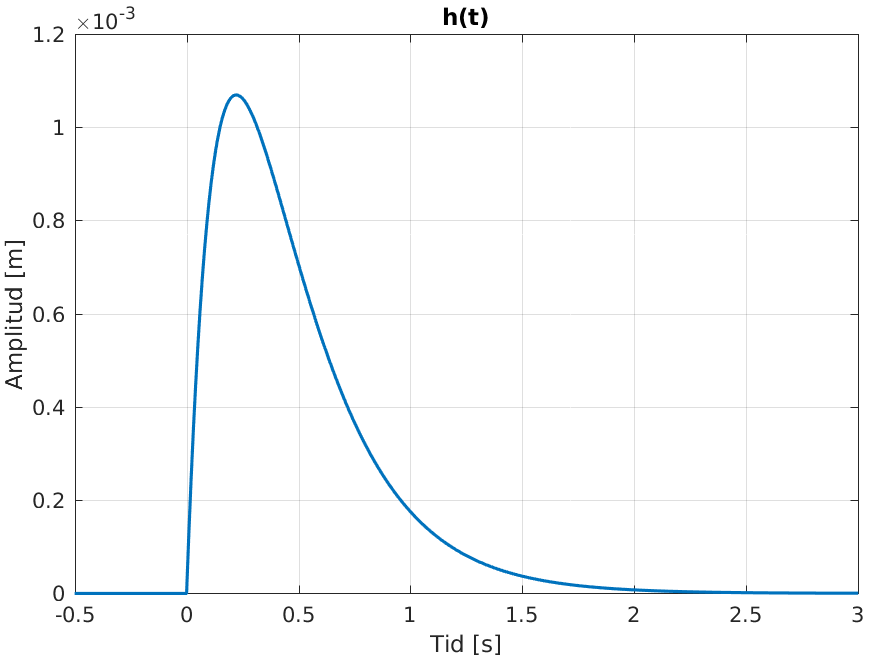
\includegraphics[scale=0.9]{bilder/impulssvar}
    \caption{Impulssvar med standardparameteruppsättning}
    \label{fig:impulssvar}
\end{figure}
Vi ser att impulssvaret snabbt avtar och efter cirka två sekunder är den ungefär tillbaka till den position där den startade. Den oscillerar inte kring viloläget vilket var den effekt vi ville ha.

\newpage
Följande figur illustrerar vad som händer då massan $m$ varierar. För att lätt kunna se vad som skiljer sig åt jämförs standardmassan med massorna $20$ kg och $200$ kg. I verkligheten skulle detta vara att personer med olika vikt står på linan.
\begin{figure}[H]
    \centering
    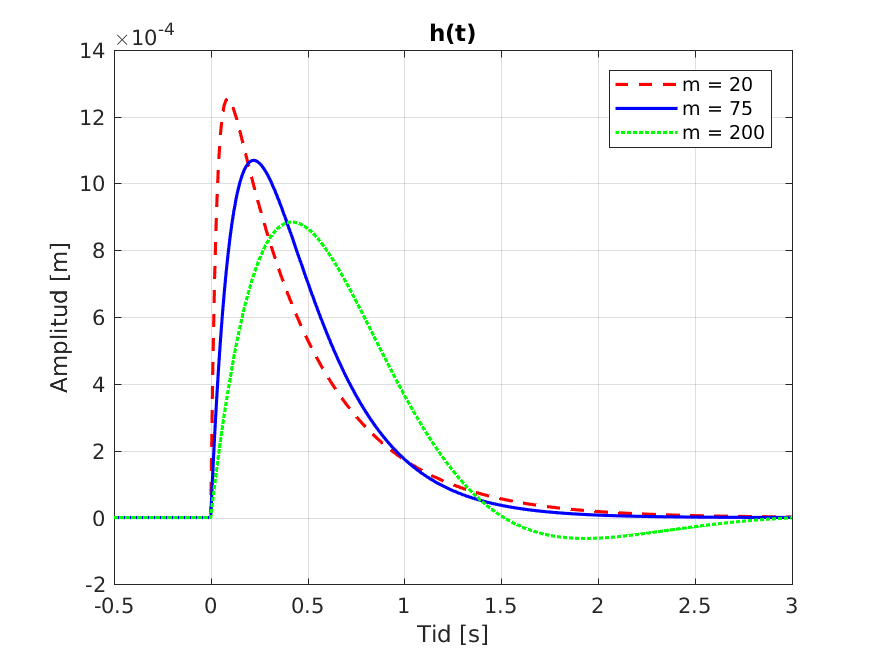
\includegraphics[scale=0.9]{bilder/impulssvar_variation_m}
    \caption{Impulssvar med varierande massa}
    \label{fig:impulssvar_variation_m}
\end{figure}
Vi ser att lättare personer når en högre amlitud och gör det snabbare än tyngre personer. Detta är rimligt eftersom tröghet gör att tyngre personer accelereras mindre av en lika stor kraft än lättare personer. Däremot innebär också trögheten att tyngre personer tar kräver mer motstånd för att stanna (då deras rörelsemängd blir högre. \textbf{Måste egentligen räkna här för att se om det stämmer. Om samma kraft påverkar en tyngre och en lättare massa är jag osäker på förhållandet mellan deras rörelsemängder. Vid samma hastighet har fetton större rörelsemängd. Men tröghet/massa i sig talar om hur mycket något "motstår" kraftpåverkan så bara det räcker för att det ska vara svårare att stoppa fetton  }).

\newpage
För att få rimliga värden på $k$ betraktas linans utdragslängd $y_0$ från mittpunkten i olika lägen. Vi studerar utdragslängerna $2$ m och $0.25$ m. Detta ger fjäderkonstanen $370$ N/m respektive $3000$ N/m. I verkligheten kan man få liknande effekt genom att spänna linan olika hårt eller flytta ändpunkterna närmre eller längre bort från varandra. Figuren nedan visar impulssvaret för de olika fjäderkonstanterna.
\begin{figure}[H] 
    \centering
    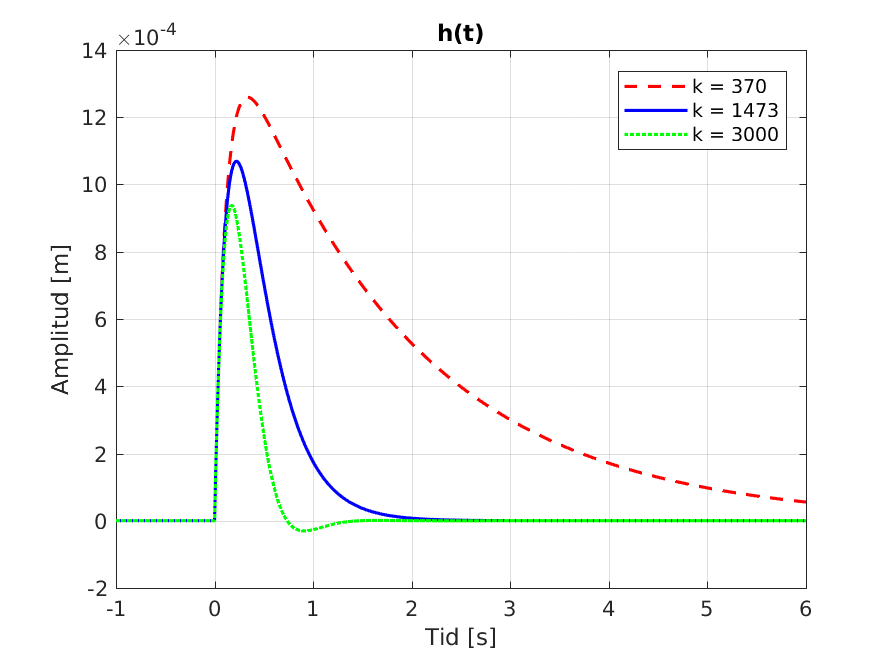
\includegraphics[scale=0.9]{bilder/impulssvar_variation_k}
    \caption{Impulssvar med varierande fjäderkonstant}
    \label{fig:impulssvar_variation_k}
\end{figure}
Här ser vi tydligt att en lägre fjäderkonstant gör att massan tar mycket längre tid att ta sig tillbaka till viloläget. Tänker man det som hur hårt linan är spänd känns det rimligt då hårdare spänd lina snabbare tar sig tillbaka till utgångsläget. 

\newpage
Nedan undersöks vad som händer då $c$ ändras. I verkligheten skulle liknande effekt fås om man ändrar materialet på linan, till exempel från ett rep till en vajer.
I figuren nedan visas impulssvaret då dämpningskonstanten halveras samt fördubblas.
\begin{figure}[H]
    \centering
    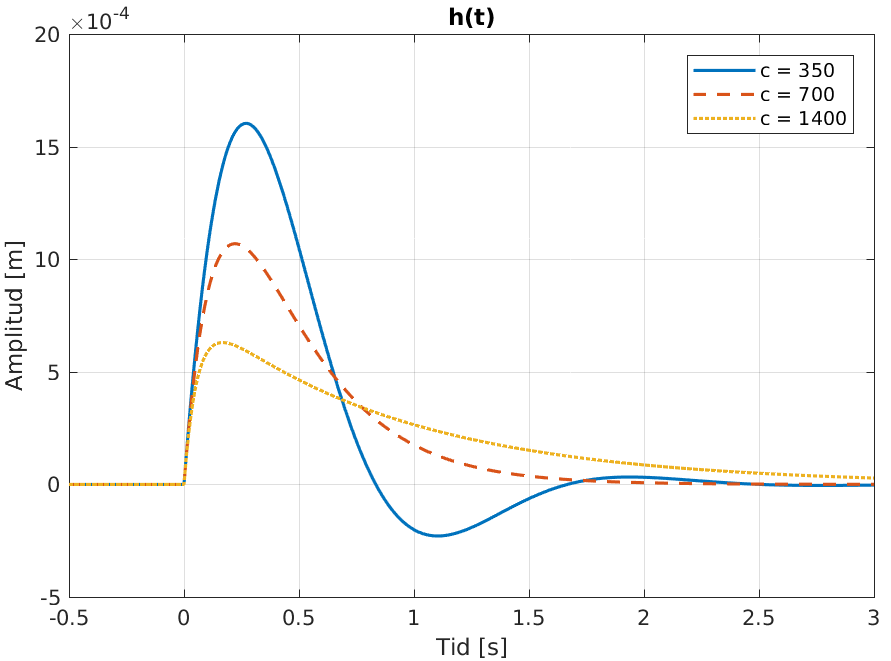
\includegraphics[scale=0.9]{bilder/impulssvar_variation_c}
    \caption{Impulssvar med varierande dämpningskonstant}
    \label{fig:impulssvar_variation_c}
\end{figure}
Vid lägre dämpningskonstant så dämpar systemet mindre och vi får en högre amplitud. Vid låg dämpning så går den också över viloläget då den inte har hunnit dämpa insignalen tillräckligt. I de andra två fallen minskar den utan oscillation och med en lägre toppamplitud desto högre dämpningskonstanten är.

\newpage
\subsection{Stegsvar}
En annan insignal vi ska studera är enhetssteget $u(t)$. Detta är en plötslig förändring av insignalen från $0$ till $1$ enligt:
$$u(t)=\begin{cases} 1, & \text{om } t \ge 0 \\ 0, & \text{om } t < 0\end{cases}$$
När ett system matas med ett enhetssteg får man stegsvaret $g(t)$ som utsignal. Detta kan i vårt system representeras av att en vikt kastas till personen på linan. Eftersom vårt system är linjärt kan denna utsignal beräknas genom att falta enhetssteget med impulssvaret som har beräknats innan. Denna uträkning kan sedan förenklas till en integral över bara impulssvaret enligt:
$$g(t)=(u*h)(t)=\int\limits_{-\infty}^{\infty}h(\tau)\,u(t-\tau)\,d\tau=\int\limits_{-\infty}^{t}h(\tau)\,d\tau$$
Våra tre typer av generella system ger upphov till tre olika impulssvar och kommer därför även ge upphov till tre olika stegsvar. För att förenkla beräkningen av dessa tre stegsvar behåller vi variabelbytena som valdes då impulsvaren beräknades. Eftersom alla impulssvar har en faktor av enhetsteget ges inget bidrag till faltningsintegralen då $t < 0$. Nedan beräknas vad som händer då $t \ge 0$.
\begin{itemize}
    \item Vid två skilda reella poler kan vi direkt integrera exponentialfunktionerna.
    $$\begin{aligned}
    g_1(t)
    &=\int\limits_{-\infty}^{t}\dfrac{1}{2m\omega_0}\bigg(e^{-(\alpha-\omega_0)\tau}-e^{-(\alpha+\omega_0)\tau}\bigg)u(\tau)\,d\tau
    \\&=\dfrac{1}{2m\omega_0}\int\limits_{0}^{t}\bigg(e^{-(\alpha-\omega_0)\tau}-e^{-(\alpha+\omega_0)\tau}\bigg)\,d\tau
    \\&=\dfrac{1}{2m\omega_0}\bigg[\frac{e^{-(\alpha+\omega_0)\tau}}{(\alpha+\omega_0)}-\frac{e^{-(\alpha-\omega_0)\tau}}{(\alpha-\omega_0)} \bigg]_{\tau=0}^{\tau=t}
    \\&=\dfrac{1}{2m\omega_0(\alpha^2-\omega_0^2)}\bigg((\alpha-\omega_0)e^{-(\alpha+\omega_0)t}-(\alpha+\omega_0)e^{-(\alpha-\omega_0)t}+2\omega_0\bigg)\end{aligned}$$
    \item Vid dubbelpol används en partiell integration för att lösa integralen.
    $$\begin{aligned}g_1(t)&=\dfrac{1}{m}\int\limits_{0}^{t}\tau e^{-\alpha \tau}\,d\tau
    \\&=\dfrac{1}{m} \bigg[\dfrac{\tau e^{-\alpha \tau}}{-\alpha}\bigg]_{\tau=0}^{\tau=t}+\dfrac{1}{m\alpha}\int\limits_{0}^{t}e^{-\alpha \tau}\,d\tau
    \\&=-\dfrac{1}{m\alpha^2}\alpha te^{-\alpha t}+\dfrac{1}{m\alpha}\bigg[\dfrac{e^{-\alpha \tau}}{-\alpha}\bigg]_{\tau=0}^{\tau=t}
    \\&=\dfrac{1}{m\alpha^2}\bigg(1-e^{-\alpha t}(\alpha t+1)\bigg)\text{\hspace{6cm}\,}\end{aligned}$$
    \newpage
    \item Vid komplexkonjugerade poler används upprepad partiell integraion tills man får tillbaka uttrycket man hade från början och kan på så sätt lösa ut stegsvaret.
    $$\begin{aligned}
    g_1(t)&=\dfrac{1}{m\omega_0}\int\limits_{0}^{t} e^{-\alpha \tau} \sin(\omega_0 \tau)\,d\tau
    \\&=\dfrac{1}{m\omega_0}\bigg[\dfrac{e^{-\alpha \tau}\sin(\omega_0 \tau)}{-\alpha}\bigg]_{\tau=0}^{\tau=t}+\dfrac{1}{m\alpha}\int\limits_{0}^{t} e^{-\alpha \tau} \cos(\omega_0\tau)\,d\tau
    \\&=-\dfrac{e^{-\alpha t}\sin(\omega_0 t)}{m\omega_0\alpha}+\dfrac{1}{m\alpha}\bigg[\dfrac{e^{-\alpha \tau}\cos(\omega_0 \tau)}{-\alpha}\bigg]_{\tau=0}^{\tau=t}-\dfrac{\omega_0}{m\alpha^2}\int\limits_{0}^{t}e^{-\alpha \tau} \sin(\omega_0 \tau)\,d\tau
    \\&=-\dfrac{e^{-\alpha t}\sin(\omega_0 t)}{m\omega_0\alpha}+\dfrac{1-e^{-\alpha t}\cos(\omega_0 t)}{m\alpha^2}-\dfrac{\omega_0^2}{\alpha^2}\,g_1(t)
    \\\Longleftrightarrow g_1(t)
    &=\dfrac{\omega_0-e^{-\alpha t}(\alpha\sin(\omega_0 t)+\omega_0\cos(\omega_0 t))}{m\omega_0(\alpha^2+\omega^2)}\end{aligned}$$
\end{itemize}
Eftersom dessa tre stegsvar bara gäller då $t\ge 0$ kommer de multipliceras med enhetssteget för ett fullständigt stegsvar enligt:
$$g(t)=g_1(t)\cdot u(t)$$
Detta ger att stegsvaren för reella poler, dubbelpol respektive komplexa polerna blir:

$\begin{cases}
g(t)=\dfrac{(\alpha-\omega_0)e^{-(\alpha+\omega_0)t}-(\alpha+\omega_0)e^{-(\alpha-\omega_0)t}+2\omega_0}{2m\omega_0(\alpha^2-\omega_0^2)}\,u(t) \\\\
g(t)=\dfrac{1-e^{-\alpha t}(\alpha t+1)}{m\alpha^2}\,u(t) \\\\
g(t)=\dfrac{\omega_0-e^{-\alpha t}(\alpha\sin(\omega_0 t)+\omega_0\cos(\omega_0 t))}{m\omega_0(\alpha^2+\omega_0^2)}\,u(t)
\end{cases}$


\newpage
\subsubsection{Variation av stegsvaret}
Vi vill nu se hur stegsvaret beter sig för olika parameteruppsättningar. För att se hur impulssvar och stegsvaret relaterar till varandra kommer vi använda samma parametrar som vi gjorde för variationen av impulssvaret. Igen så börjar vi kolla vad som händer med vår standardparameteruppsättning, alltså då $m = 75$ kg, $k=1473$ N/m och $c=700$ kg/s. Detta göras nedan i figuren.
\begin{figure}[H]
    \centering
    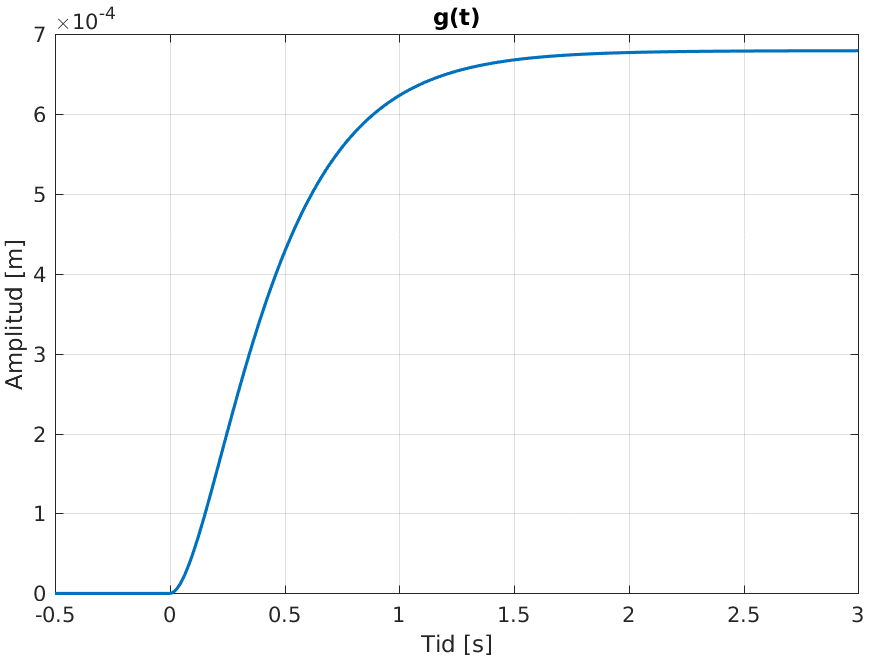
\includegraphics[scale=0.9]{bilder/stegsvar}
    \caption{Stegsvar med standardparameteruppsättning}
    \label{fig:stegsvar}
\end{figure}
Vi ser att efter cirka 1.5 sekunder har den nått ett nytt läge längre ned. Detta görs utan ocellation kring de nya viloläget. Detta skulle i verkligheten vara som  att kasta en vikt på ungefär $0.1$ kg till lindansren.

\newpage
Nu vill vi kolla vad som händer då massan förändras. Igen så används massorna $20$ kg och $200$ kg som representerar en lättare och tyngre person på linan.
\begin{figure}[H]
    \centering
    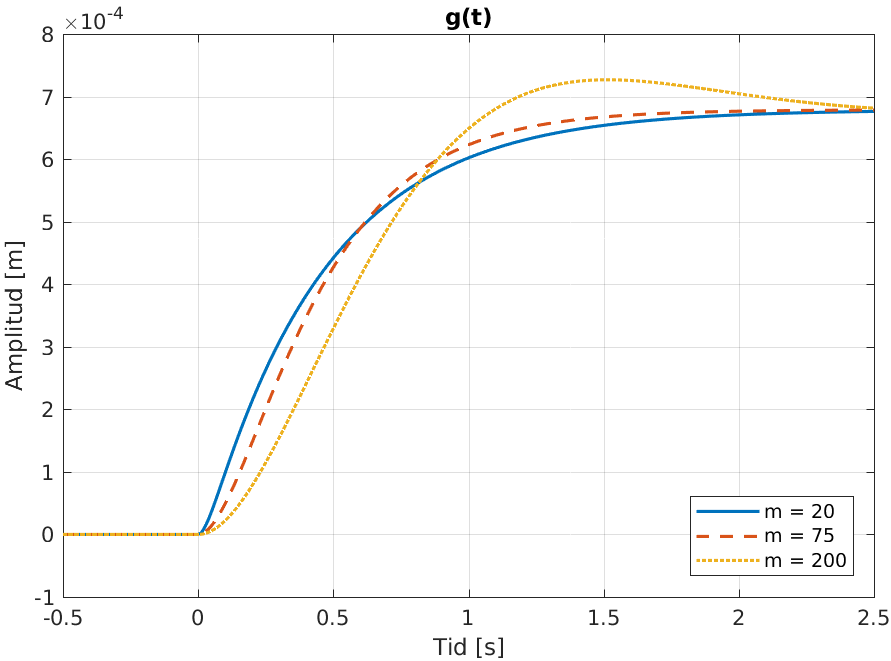
\includegraphics[scale=0.9]{bilder/stegsvar_variation_m}
    \caption{Stegsvar med varierande massa}
    \label{fig:stegsvar_variation_m}
\end{figure}
Här ser inte så stor skillnad på de 3 olika massorna, de närmar sig de nya höjdläget vid ungefär samma tidpunkt. Den tyngre massan tar längre tid på sig att börja röra sig men kommer också längre ned än de andra två och skapar också oscillation.
Vi kan också notera att massan inte påverkar nivåkonstanten då dessa går mot samma jämviktsläge.

\newpage
Härnäst ska fjäderkonstanen variera mellan $370$, $1473$ och $3000$, vilket gäller då linan är utdragen $2$ m, $0.5$ m respektive $0.25$ m från mittpunkten. Figuren nedan visar hur stegsvaret beter sig vid dessa värden.
\begin{figure}[H]
    \centering
    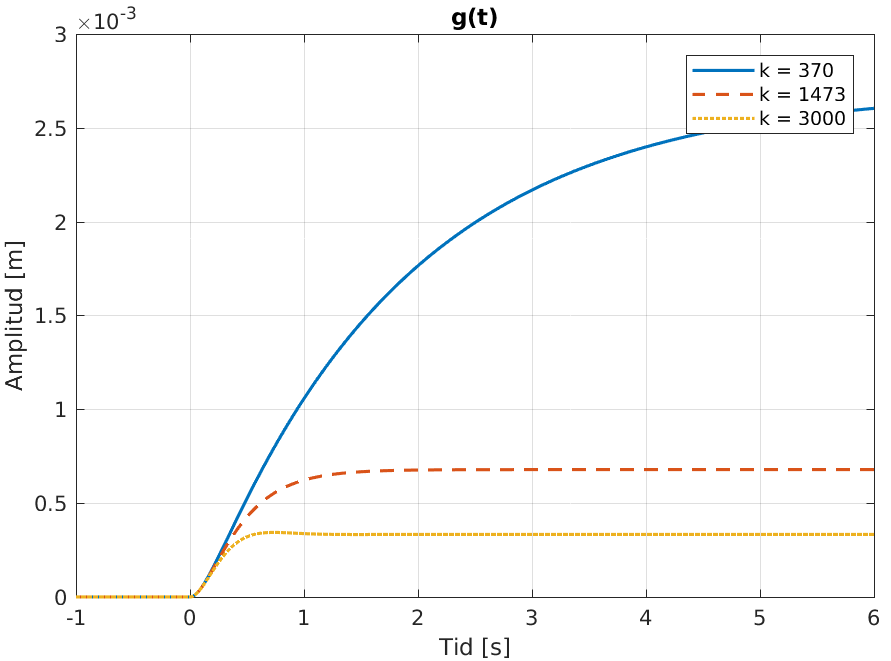
\includegraphics[scale=0.9]{bilder/stegsvar_variation_k}
    \caption{Stegsvar med varierande fjäderkonstant}
    \label{fig:stegsvar_variation_k}
\end{figure}
Vi ser direkt att $k$ påverkar nivåkonstanten och alltså hur långt ned personen kan åka ned med den kraft som appliceras. Som för impulssvaret tar en mindre fjäderkonstant längre tid att komma till ett plant läge. Vi kan också notera en liten övergång över det nya läget då $k=3000$.

\textbf{extremt rimligt om man ser fjäderkonstanten som hur ''tight'' linan är spänd. nämn om det om detta faktiskt stämmer}
\newpage
Sist varierar vi dämpningskonstanten $c$ med att både halvera och dubblera den. Denna graf visas nedan.
\begin{figure}[H]
    \centering
    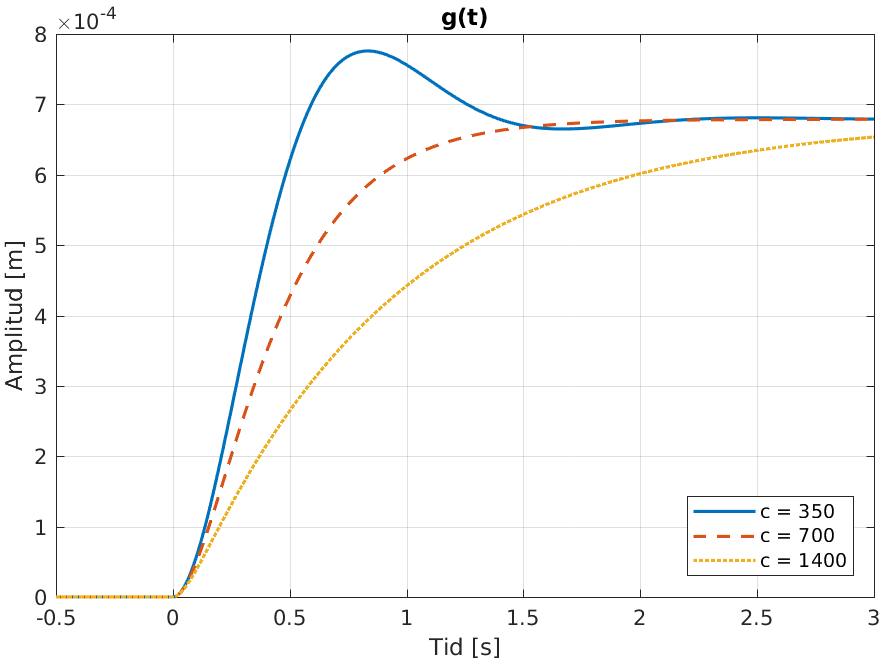
\includegraphics[scale=0.9]{bilder/stegsvar_variation_c}
    \caption{Stegsvar med varierande dämpningskonstant}
    \label{fig:stegsvar_variation_c}
\end{figure}
Likt impulssvaret så leder en hög dämpningskonstant till en kraftigare dämpning. Intressant nog så kommer stegsvaret för de lägre dämpningskonstanerna snabbare till det nya läget än den höga konstanten. 

\newpage
\subsection{Stabilitet}
För att bestämma systemets frekvensfunktion måste impulssvaret vara fouriertransformerbart vilket kräver att systemet är stabilt. Ett stabilt system är ett system där begränsade insignaler alltid ger begränsade utsignaler. För att bestämma om ett system är stabilt eller inte finns olika tillvägagångssätt. Ett sätt att bestämma detta är att titta på impulssvaret. Om impulssvaret är absolutintegrerbart så är systemet stabilt. Att impulssvaret är absolutintegrerbart innebär att:
$$\int\limits_{-\infty}^{\infty}\big|h(t)\big|\,dt < \infty$$
Ett annat sätt att bestämma om systemet är stabilt är att kolla på konvergensområdet för systemfunktionen. Om den imaginära axeln alltså $j\omega$-axeln är i konvergensområdet så är systmet stabilt.
Detta gäller alltid för vårt system som kan ses i pol-nollställediagramen för systemfunktionen i kapitel $2.2.1$. Egentligen krävs också att $m,k,c>0$ men detta har antagits för att modellen ens ska ge mening.
\subsection{Frekvensfunktion}
För att se hur vårt system påverkar signaler av olika frekvenser kommer vi betrakta systemets frekvenskfunktion $H(\omega)$.
Frekvensfunktionen är Fouriertransformen av impulssvaret $h(t)$. För att Fouriertransformen ska existera krävs att systemet är stabilt vilket visades i föregående kapitel. Vidare är Fouriertransformen ett specialfall av Laplacetransformen där variablen $s = j\omega$. Frekvensfunktionen har alltså bara den reella vinkelfrekvensen $\omega$ som argument. Med insättning av $s = j\omega$ i systemfunktionen $H(s)$ fås: 

$$H(\omega)=H(s)\bigg\rvert_{s=j\omega}=\dfrac{1}{m(j\omega)^2+cj\omega+k}$$

\newpage
\subsection{Amplitudkaraktäristik}
Vi kommer nu titta hur systemet påverker amplituden av utsignalen beroende på frekvensen av insignalen. Amplitudkaraktäristiken är absolutbelopet av frekvensfunktionen och visar hur systemet dämpar och förstärker vissa signaler. 
$$\big|H(\omega)\big|=\dfrac{1}{\Big|\,m(j\omega)^2+cj\omega+k\,\Big|}=\dfrac{1}{\sqrt{\big(k-m\,\omega^2\big)^2+\big(c\,\omega\big)^2}}$$
Det allra första som kommer studeras vad som händer med amplituder för vår standardparameteruppsättning, alltså då $m=75$ kg, $k=1473$ N/m och $c=700$ kg/s. Detta visas i figuren nedan.
\begin{figure}[H]
    \centering
    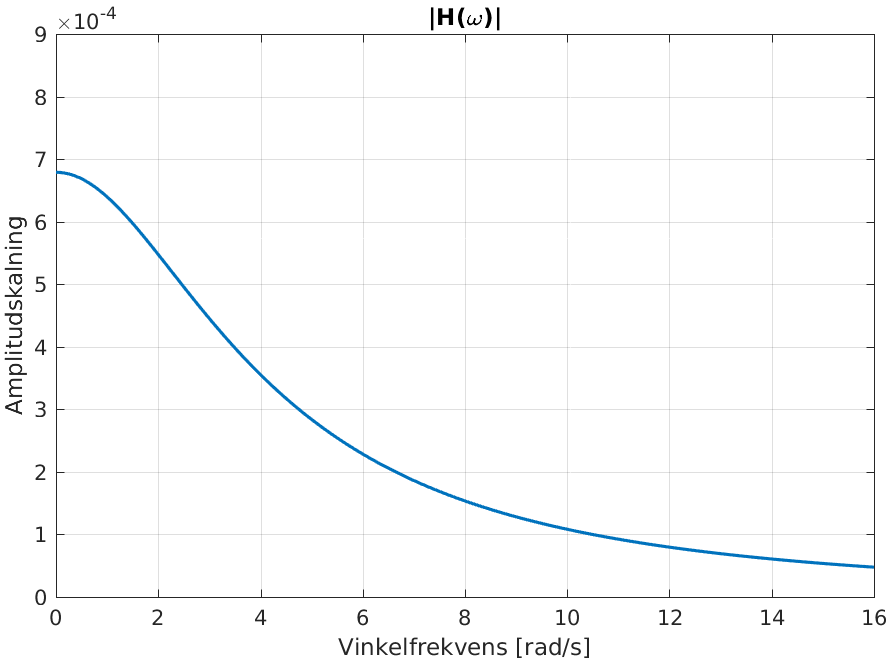
\includegraphics[scale=0.9]{bilder/amplitudkaraktaristik}
    \caption{Amplitudkaraktäristik med standardparameteruppsättning}
    \label{fig:amplitudkaraktaristik}
\end{figure}
Vi ser att systemet släpper igenom låga frekvenser och dämpar höga frekvenser. Detta system beter sig som ett lågpassfilter.
Då vi har olika enheter på insignal och utsignal, en kraft respektive en längd, är det svårt att tolka hur mycket som faktist förstärks eller dämpas vid en viss vinkelfrekvens (\textbf{detta behvöer inte nämnas}). Vi kan utifrån grafen se att gränsvinkelfrekvensen är ungefär $2.5$ rad/s, alltså då:
$$\big|H(\omega)\big|=\dfrac{max\Big\{\big|H(\omega)\big|\Big\}}{\sqrt{2}}\approx \frac{7}{\sqrt{2}} \approx 5$$
\newpage
\textbf{Ehhhh förslag: hoppa över de två första graferna och ta bara den med c. Anledning? Det finns inte så mycket att prata om som inte redan sagts samt sidobrist}

\begin{figure}[H]
    \centering
    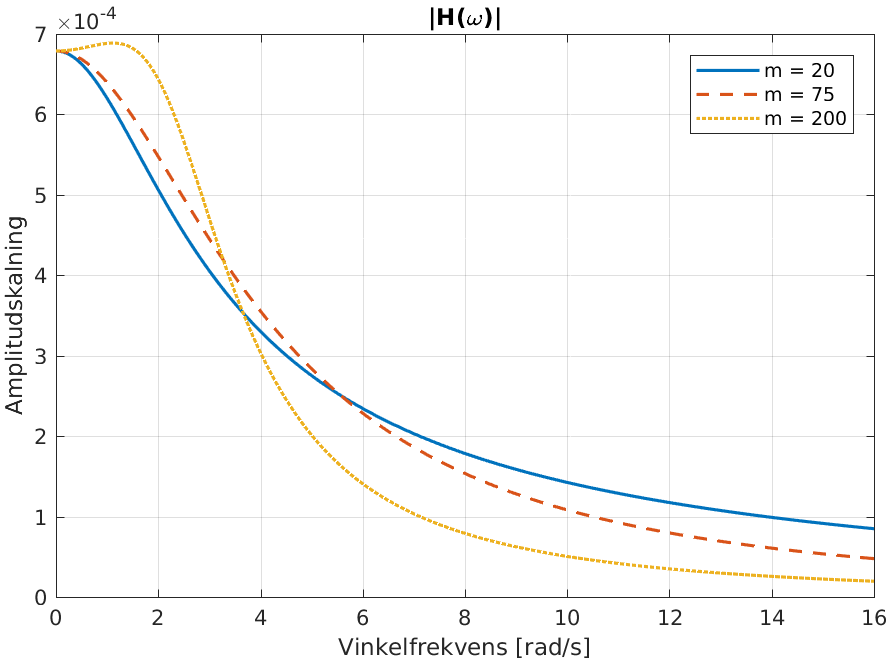
\includegraphics[scale=0.9]{bilder/amplitudkaraktaristik_variation_m}
    \caption{Amplitudkaraktäristik med varierande massa}
    \label{fig:amplitudkaraktaristik_variation_m}
\end{figure}

\newpage
\begin{figure}[H]
    \centering
    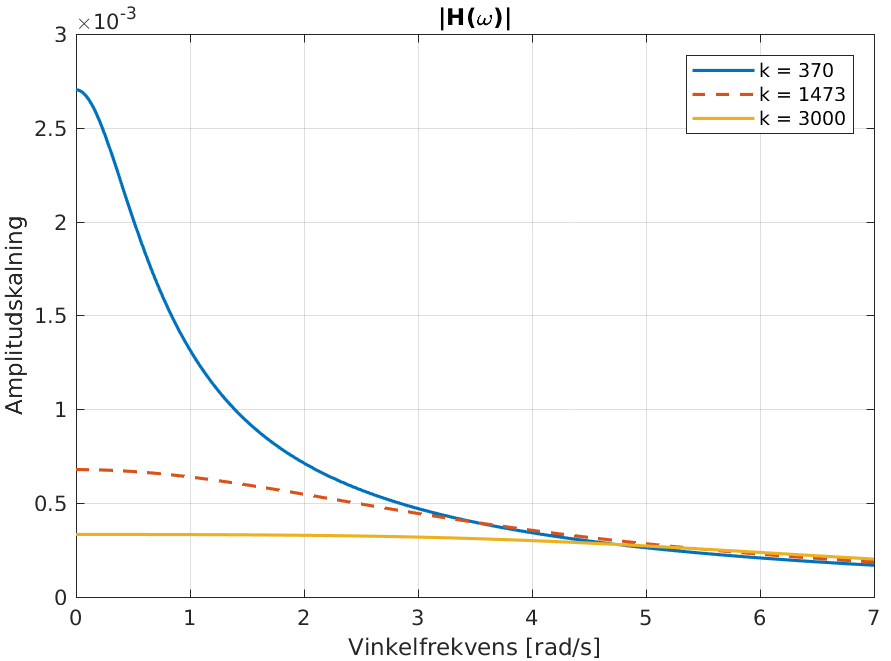
\includegraphics[scale=0.9]{bilder/amplitudkaraktaristik_variation_k}
    \caption{Amplitudkaraktäristik med varierande fjäderkonstant}
    \label{fig:amplitudkaraktaristik_variation_k}
\end{figure}

\newpage
Härnäst kommer vi hur se hur amplitudkaraktäristiken beter sig när dämpningskonstanten ändras. Igen väljer vi att halvera och dubblera konstanten vilket visas i figuren nedan.  
\begin{figure}[H]
    \centering
    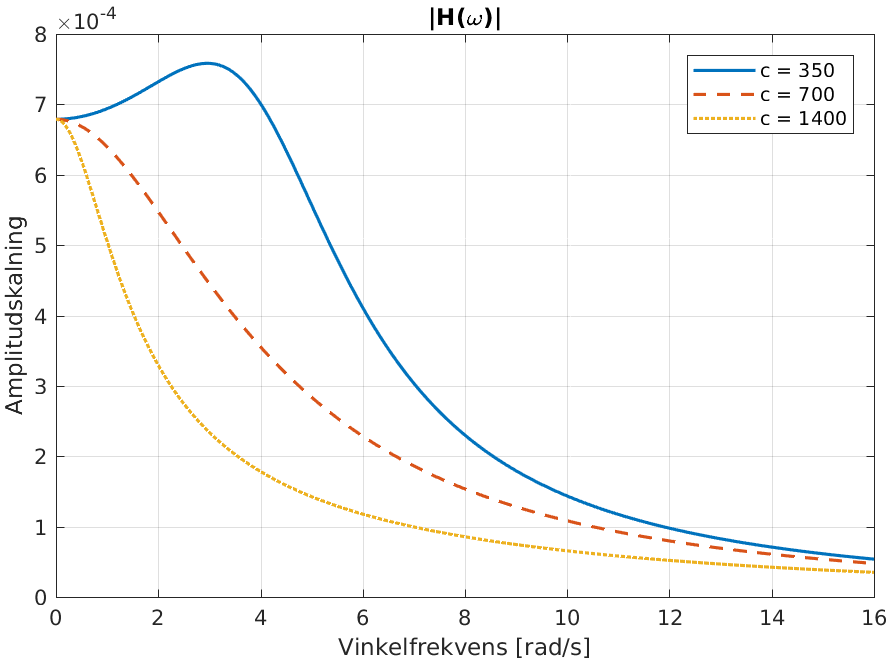
\includegraphics[scale=0.9]{bilder/amplitudkaraktaristik_variation_c}
    \caption{Amplitudkaraktäristik med varierande dämpningskonstant}
    \label{fig:amplitudkaraktaristik_variation_c}
\end{figure}
Vi ser generellt att en högre dämpningskonstant dämpar mer för alla frekvenser. Vid en lägre dämpningskonstant bildas komplexkonjugerade poler i frekvensdomänen vilker betyder att toppen av amplitudkaraktäristiken flyttas åt höger. I det fallet får vi en nollskild resonansfrekvens, vilket i grafen kan avläsas vara ungefär $3$ rad/s. 

\newpage
\subsection{Faskaraktäristik}
Faskaraktäristiken beskriver hur mycket systemet förskjuter en signal i fas beroende på frekvensen. Denna kan tas fram genom att ta argumentet för frekvensfunktionen enligt:
$$arg\big\{H(w)\big\}=\arg\big\{1\big\}-\arg\big\{k-m\omega^2+jc\,\omega\big\}$$
$$=\begin{cases}
-\arctan\bigg(\dfrac{c\,\omega}{k-m\omega^2}\bigg), & \text{om } k-m\omega^2 > 0  \\\\
-\arctan\bigg(\dfrac{c\,\omega}{k-m\omega^2}\bigg)-\pi, & \text{om } k-m\omega^2 < 0 \\\\ 
-\dfrac{\pi}{2}, & \text{om } k-m\omega^2 = 0 
\end{cases}$$
I grafen nedan visas faskaraktäristiken för vår standardparameteruppsättning.
\begin{figure}[H]
    \centering
    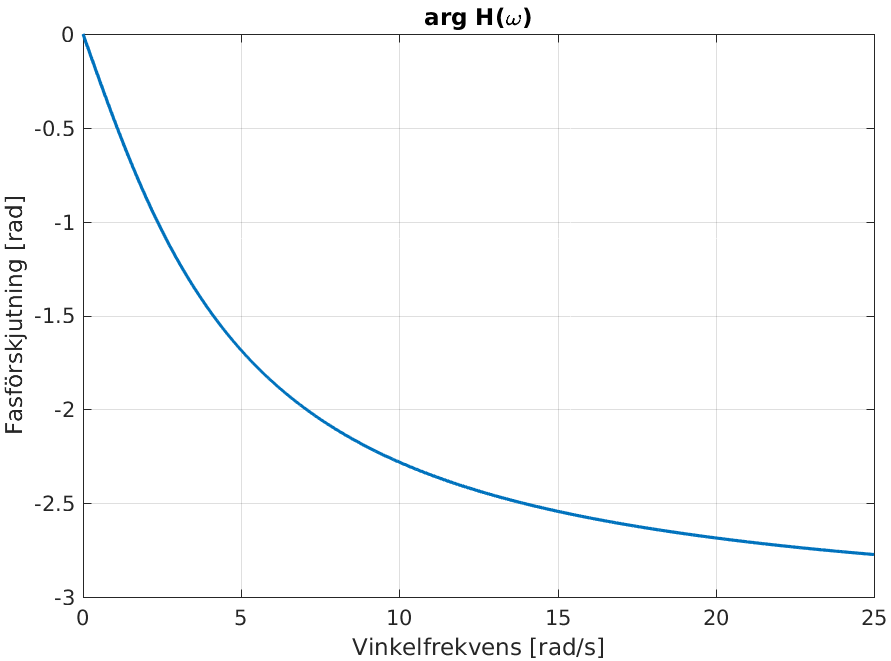
\includegraphics[scale=0.75]{bilder/faskaraktaristik}
    \caption{Faskaraktäristik med standardparameteruppsättning}
    \label{fig:faskaraktaristik}
\end{figure}
Vi ser att vårt system fastförskjuter signaler med högre frekvenser mer än lägre. Man kan alltså säga att systemet reagerar bättre på långsamma förändringar än snabba.
Argumentet kommer i detta fall gå mot $-\pi$ då frekvensen går mot oändligheten. Detta kan bevisas då för det för stora $\omega$  gäller att:
$$\lim_{\omega\to\infty}-\arctan\bigg(\dfrac{c\,\omega}{k-m\omega^2}\bigg)-\pi=
\lim_{\omega\to\infty}-\arctan\Bigg(\dfrac{1}{\omega}\cdot\frac{c}{\frac{k}{\omega^2}-m}\Bigg)-\pi=-\arctan(0)-\pi=-\pi$$
Då faskaratäristiken inte är intressant för vårt system kommer vi inte analysera den något yttligare.
\newpage
\subsection{Stationära sinussignaler}
När ett LTI-system matas med en godtycklig sinusfunktion som insignal, till exempel följande insignal $x(t)$:
$$x(t)=A\sin(\omega_0t)$$
får vi en utsignal $y(t)$ som kan beräknas med hjälp av frekvensfunktionen $H(\omega)$ enligt:
$$y(t)=A\,\big|H(\omega_0)\big|\sin\big(\omega_0t+\arg\big\{H(\omega_0)\big\}\big)$$
Man får alltså att utsignalen är en amplitudskalad för fastförskjuten verision av insignalen.
Detta gör det väldigt lätt att beräkna utsignalen om insignalen är en sinusfunktion och frekvensfunktion är bestämd. Vi ska nu se hur vårt system reagerar på olika typer av sinusfunktioner med olika frekvenser.


--------------------------------------------------------------------

analysera två stationära sinussignaler  med, för just ert system, väl valda/motiverade och intressanta frekvenser.

Mina förslag: resonans och en vanligt gångtakt hos en lindansare (vi får pröva och se på videos). Alt. (resonans + hög frek + låg frek)
\textbf{Ev. borde vil kolla på stegsvar med skalad input typ 10 eller 100 N in. 1 N är ju typ ingenting}

Fråga Lasse?
\subsubsection{Resonans}
oh no vårt system har ingen responansfrekvens för att det är att lågpassfilter, man kan ändra detta genom att ändra systemparamterarna med det känns fel.

\textbf{Njaeoea, g  ul i fig 16 och blå i fig 18 har resonanser och är lågpass. Vi saknar resonans pga sys.parametrarna, men inte för att det är ett LP}
\subsubsection{Gångtakt}

\newpage
\subsection{SAKER SOM SKA KOLLAS DÅ ALLT ÄR KLART}
\begin{itemize}
    \item SKRIV IMPULSSVARET ISTÄLLET FÖR BARA $h(t)$ I TEXT1!!!!!!!!
    \item Vi blandar tex ''3'' och ''tre'' lite överallt. Använd en av dom (helst den som är korrekt http://dinsvenska.se/datum-tid-och-rakneord/ska-man-skriva-tal-med-siffror-eller-bokstaver/)
    \item Förslag för förtydligande: Döpa om alla $h(t)$ till $h_r(t)$, $h_d(t)$  och $h_k(t)$ för reella, dubbel och komplex, alt. $h_1(t), h_2(t), h_3(t)$
    \item Kolla ekvationerna, framför stora snedsträck används ibland ''='' och ibland ''$\Longleftrightarrow$''. Tror att vissa av dessa är fel.
    \item Ska vi använda dubbel- eller enkelpilar? 
    \item Fixa storleken på alla formler i rapporten
    \item Lös kommentarerna i kapitel 1.3 angående friktionen.
    \item Lägg till text för att läsaren ska tolka och förstå bättre under Bevis av linjäritet.
    \item Fråga en annan grupp om de kan läsa vår rapport och ge kommentarer (i utbyte att vi läser deras)
    \item Lägg till radbrytning där det ser snyggt ut
    \item Läs igenom i grupp
    \item Skriv ut och läs igen
\end{itemize}